\documentclass[12pt]{article}

\usepackage[T1]{fontenc}
\usepackage[utf8]{inputenc}
\usepackage[russian]{babel}

\usepackage{amsmath}
\usepackage{float}
\usepackage{tabularx}

% page margin
\usepackage[top=2cm, bottom=2cm, left=2cm, right=2cm]{geometry}

\usepackage{graphicx}

\begin{document}

\begin{figure}
	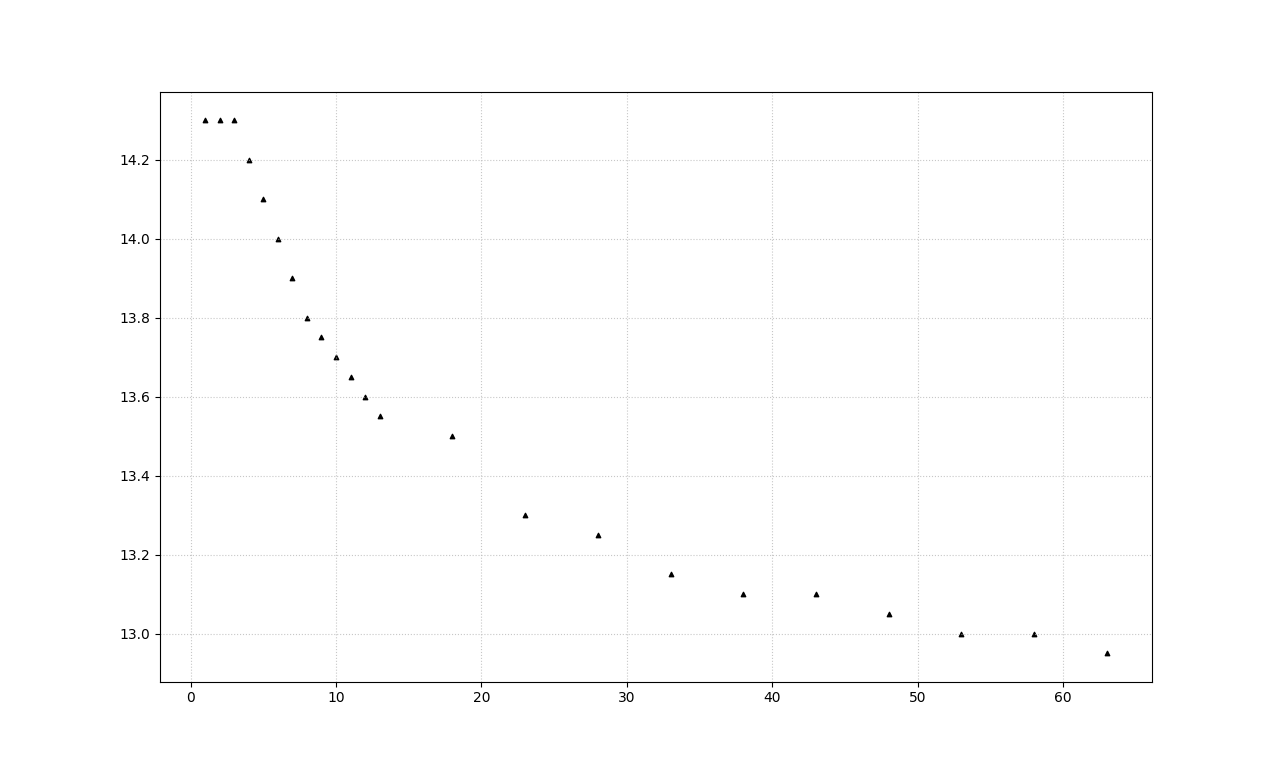
\includegraphics[width = \linewidth]{../isotherm.png}
	\caption{Изотерма кристаллизации}
\end{figure}

\begin{figure}
	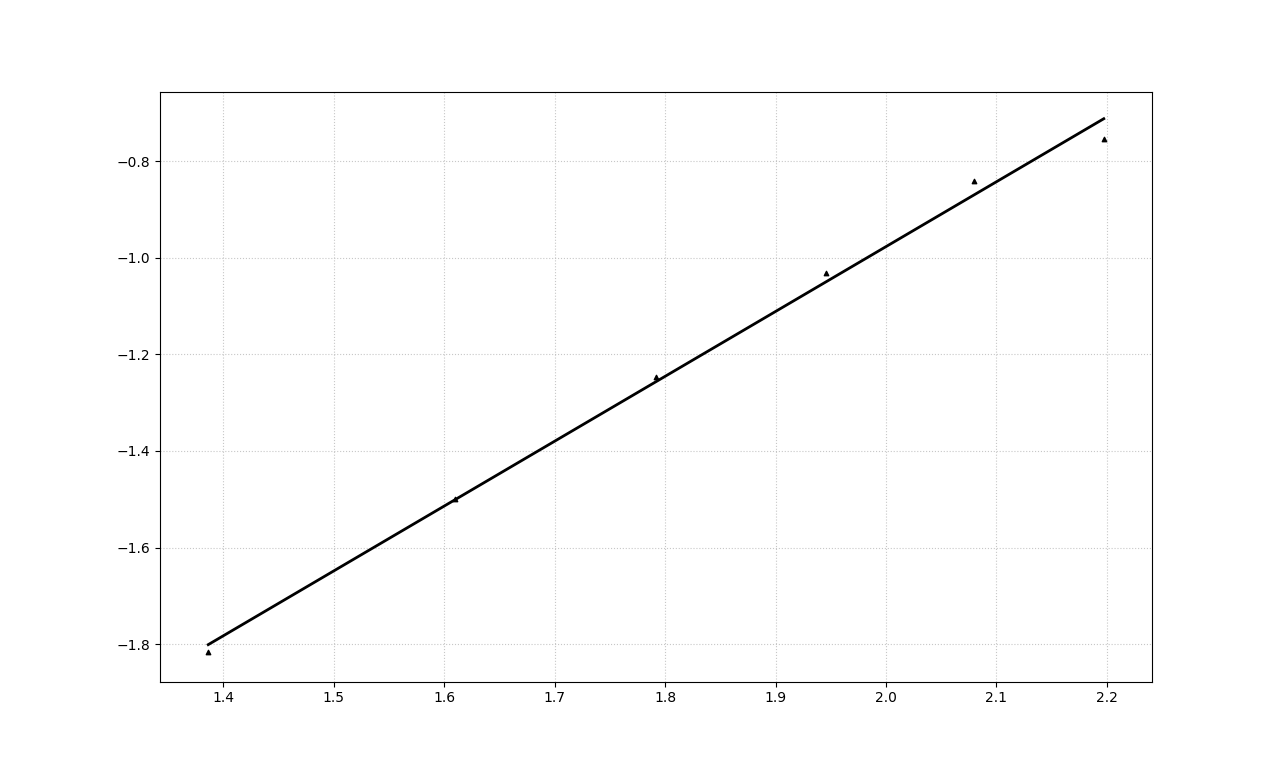
\includegraphics[width = \linewidth]{../linear.png}
	\caption{Линеаризация участка резкого падения на кинетической кривой}
\end{figure}

\end{document}

